\documentclass[1p]{elsarticle_modified}
%\bibliographystyle{elsarticle-num}

%\usepackage[colorlinks]{hyperref}
%\usepackage{abbrmath_seonhwa} %\Abb, \Ascr, \Acal ,\Abf, \Afrak
\usepackage{amsfonts}
\usepackage{amssymb}
\usepackage{amsmath}
\usepackage{amsthm}
\usepackage{scalefnt}
\usepackage{amsbsy}
\usepackage{kotex}
\usepackage{caption}
\usepackage{subfig}
\usepackage{color}
\usepackage{graphicx}
\usepackage{xcolor} %% white, black, red, green, blue, cyan, magenta, yellow
\usepackage{float}
\usepackage{setspace}
\usepackage{hyperref}

\usepackage{tikz}
\usetikzlibrary{arrows}

\usepackage{multirow}
\usepackage{array} % fixed length table
\usepackage{hhline}

%%%%%%%%%%%%%%%%%%%%%
\makeatletter
\renewcommand*\env@matrix[1][\arraystretch]{%
	\edef\arraystretch{#1}%
	\hskip -\arraycolsep
	\let\@ifnextchar\new@ifnextchar
	\array{*\c@MaxMatrixCols c}}
\makeatother %https://tex.stackexchange.com/questions/14071/how-can-i-increase-the-line-spacing-in-a-matrix
%%%%%%%%%%%%%%%

\usepackage[normalem]{ulem}

\newcommand{\msout}[1]{\ifmmode\text{\sout{\ensuremath{#1}}}\else\sout{#1}\fi}
%SOURCE: \msout is \stkout macro in https://tex.stackexchange.com/questions/20609/strikeout-in-math-mode

\newcommand{\cancel}[1]{
	\ifmmode
	{\color{red}\msout{#1}}
	\else
	{\color{red}\sout{#1}}
	\fi
}

\newcommand{\add}[1]{
	{\color{blue}\uwave{#1}}
}

\newcommand{\replace}[2]{
	\ifmmode
	{\color{red}\msout{#1}}{\color{blue}\uwave{#2}}
	\else
	{\color{red}\sout{#1}}{\color{blue}\uwave{#2}}
	\fi
}

\newcommand{\Sol}{\mathcal{S}} %segment
\newcommand{\D}{D} %diagram
\newcommand{\A}{\mathcal{A}} %arc


%%%%%%%%%%%%%%%%%%%%%%%%%%%%%5 test

\def\sl{\operatorname{\textup{SL}}(2,\Cbb)}
\def\psl{\operatorname{\textup{PSL}}(2,\Cbb)}
\def\quan{\mkern 1mu \triangleright \mkern 1mu}

\theoremstyle{definition}
\newtheorem{thm}{Theorem}[section]
\newtheorem{prop}[thm]{Proposition}
\newtheorem{lem}[thm]{Lemma}
\newtheorem{ques}[thm]{Question}
\newtheorem{cor}[thm]{Corollary}
\newtheorem{defn}[thm]{Definition}
\newtheorem{exam}[thm]{Example}
\newtheorem{rmk}[thm]{Remark}
\newtheorem{alg}[thm]{Algorithm}

\newcommand{\I}{\sqrt{-1}}
\begin{document}

%\begin{frontmatter}
%
%\title{Boundary parabolic representations of knots up to 8 crossings}
%
%%% Group authors per affiliation:
%\author{Yunhi Cho} 
%\address{Department of Mathematics, University of Seoul, Seoul, Korea}
%\ead{yhcho@uos.ac.kr}
%
%
%\author{Seonhwa Kim} %\fnref{s_kim}}
%\address{Center for Geometry and Physics, Institute for Basic Science, Pohang, 37673, Korea}
%\ead{ryeona17@ibs.re.kr}
%
%\author{Hyuk Kim}
%\address{Department of Mathematical Sciences, Seoul National University, Seoul 08826, Korea}
%\ead{hyukkim@snu.ac.kr}
%
%\author{Seokbeom Yoon}
%\address{Department of Mathematical Sciences, Seoul National University, Seoul, 08826,  Korea}
%\ead{sbyoon15@snu.ac.kr}
%
%\begin{abstract}
%We find all boundary parabolic representation of knots up to 8 crossings.
%
%\end{abstract}
%\begin{keyword}
%    \MSC[2010] 57M25 
%\end{keyword}
%
%\end{frontmatter}

%\linenumbers
%\tableofcontents
%
\newcommand\colored[1]{\textcolor{white}{\rule[-0.35ex]{0.8em}{1.4ex}}\kern-0.8em\color{red} #1}%
%\newcommand\colored[1]{\textcolor{white}{ #1}\kern-2.17ex	\textcolor{white}{ #1}\kern-1.81ex	\textcolor{white}{ #1}\kern-2.15ex\color{red}#1	}

{\Large $\underline{12a_{0858}~(K12a_{0858})}$}

\setlength{\tabcolsep}{10pt}
\renewcommand{\arraystretch}{1.6}
\vspace{1cm}\begin{tabular}{m{100pt}>{\centering\arraybackslash}m{274pt}}
\multirow{5}{120pt}{
	\centering
	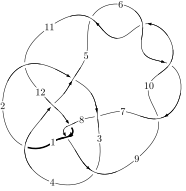
\includegraphics[width=112pt]{../../../GIT/diagram.site/Diagrams/png/1659_12a_0858.png}\\
\ \ \ A knot diagram\footnotemark}&
\allowdisplaybreaks
\textbf{Linearized knot diagam} \\
\cline{2-2}
 &
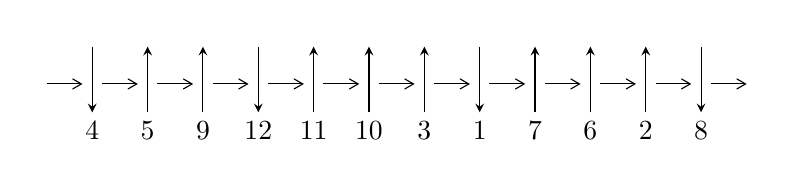
\begin{tikzpicture}[x=20pt, y=17pt]
	% nodes
	\node (C0) at (0, 0) {};
	\node (C1) at (1, 0) {};
	\node (C1U) at (1, +1) {};
	\node (C1D) at (1, -1) {4};

	\node (C2) at (2, 0) {};
	\node (C2U) at (2, +1) {};
	\node (C2D) at (2, -1) {5};

	\node (C3) at (3, 0) {};
	\node (C3U) at (3, +1) {};
	\node (C3D) at (3, -1) {9};

	\node (C4) at (4, 0) {};
	\node (C4U) at (4, +1) {};
	\node (C4D) at (4, -1) {12};

	\node (C5) at (5, 0) {};
	\node (C5U) at (5, +1) {};
	\node (C5D) at (5, -1) {11};

	\node (C6) at (6, 0) {};
	\node (C6U) at (6, +1) {};
	\node (C6D) at (6, -1) {10};

	\node (C7) at (7, 0) {};
	\node (C7U) at (7, +1) {};
	\node (C7D) at (7, -1) {3};

	\node (C8) at (8, 0) {};
	\node (C8U) at (8, +1) {};
	\node (C8D) at (8, -1) {1};

	\node (C9) at (9, 0) {};
	\node (C9U) at (9, +1) {};
	\node (C9D) at (9, -1) {7};

	\node (C10) at (10, 0) {};
	\node (C10U) at (10, +1) {};
	\node (C10D) at (10, -1) {6};

	\node (C11) at (11, 0) {};
	\node (C11U) at (11, +1) {};
	\node (C11D) at (11, -1) {2};

	\node (C12) at (12, 0) {};
	\node (C12U) at (12, +1) {};
	\node (C12D) at (12, -1) {8};
	\node (C13) at (13, 0) {};

	% arrows
	\draw[->,>={angle 60}]
	(C0) edge (C1) (C1) edge (C2) (C2) edge (C3) (C3) edge (C4) (C4) edge (C5) (C5) edge (C6) (C6) edge (C7) (C7) edge (C8) (C8) edge (C9) (C9) edge (C10) (C10) edge (C11) (C11) edge (C12) (C12) edge (C13) ;	\draw[->,>=stealth]
	(C1U) edge (C1D) (C2D) edge (C2U) (C3D) edge (C3U) (C4U) edge (C4D) (C5D) edge (C5U) (C6D) edge (C6U) (C7D) edge (C7U) (C8U) edge (C8D) (C9D) edge (C9U) (C10D) edge (C10U) (C11D) edge (C11U) (C12U) edge (C12D) ;
	\end{tikzpicture} \\
\hhline{~~} \\& 
\textbf{Solving Sequence} \\ \cline{2-2} 
 &
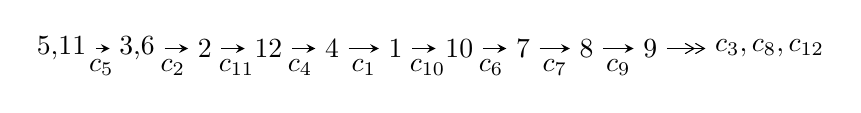
\begin{tikzpicture}[x=23pt, y=7pt]
	% node
	\node (A0) at (-1/8, 0) {5,11};
	\node (A1) at (17/16, 0) {3,6};
	\node (A2) at (17/8, 0) {2};
	\node (A3) at (25/8, 0) {12};
	\node (A4) at (33/8, 0) {4};
	\node (A5) at (41/8, 0) {1};
	\node (A6) at (49/8, 0) {10};
	\node (A7) at (57/8, 0) {7};
	\node (A8) at (65/8, 0) {8};
	\node (A9) at (73/8, 0) {9};
	\node (C1) at (1/2, -1) {$c_{5}$};
	\node (C2) at (13/8, -1) {$c_{2}$};
	\node (C3) at (21/8, -1) {$c_{11}$};
	\node (C4) at (29/8, -1) {$c_{4}$};
	\node (C5) at (37/8, -1) {$c_{1}$};
	\node (C6) at (45/8, -1) {$c_{10}$};
	\node (C7) at (53/8, -1) {$c_{6}$};
	\node (C8) at (61/8, -1) {$c_{7}$};
	\node (C9) at (69/8, -1) {$c_{9}$};
	\node (A10) at (11, 0) {$c_{3},c_{8},c_{12}$};

	% edge
	\draw[->,>=stealth]	
	(A0) edge (A1) (A1) edge (A2) (A2) edge (A3) (A3) edge (A4) (A4) edge (A5) (A5) edge (A6) (A6) edge (A7) (A7) edge (A8) (A8) edge (A9) ;
	\draw[->>,>={angle 60}]	
	(A9) edge (A10);
\end{tikzpicture} \\ 

\end{tabular} \\

\footnotetext{
The image of knot diagram is generated by the software ``\textbf{Draw programme}" developed by Andrew Bartholomew(\url{http://www.layer8.co.uk/maths/draw/index.htm\#Running-draw}), where we modified some parts for our purpose(\url{https://github.com/CATsTAILs/LinksPainter}).
}\phantom \\ \newline 
\centering \textbf{Ideals for irreducible components\footnotemark of $X_{\text{par}}$} 
 
\begin{align*}
I^u_{1}&=\langle 
-4.29209\times10^{154} u^{103}-9.15492\times10^{154} u^{102}+\cdots+1.10622\times10^{155} b-5.83673\times10^{155},\\
\phantom{I^u_{1}}&\phantom{= \langle  }-5.85136\times10^{155} u^{103}-1.74496\times10^{156} u^{102}+\cdots+1.10622\times10^{155} a-7.67740\times10^{156},\\
\phantom{I^u_{1}}&\phantom{= \langle  }u^{104}+3 u^{103}+\cdots+31 u+1\rangle \\
I^u_{2}&=\langle 
- u^{21}- u^{20}+\cdots+b-3,\;2 u^{21}+4 u^{20}+\cdots+a+3,\;u^{22}+2 u^{21}+\cdots+8 u+1\rangle \\
\\
\end{align*}
\raggedright * 2 irreducible components of $\dim_{\mathbb{C}}=0$, with total 126 representations.\\
\footnotetext{All coefficients of polynomials are rational numbers. But the coefficients are sometimes approximated in decimal forms when there is not enough margin.}
\newpage
\renewcommand{\arraystretch}{1}
\centering \section*{I. $I^u_{1}= \langle -4.29\times10^{154} u^{103}-9.15\times10^{154} u^{102}+\cdots+1.11\times10^{155} b-5.84\times10^{155},\;-5.85\times10^{155} u^{103}-1.74\times10^{156} u^{102}+\cdots+1.11\times10^{155} a-7.68\times10^{156},\;u^{104}+3 u^{103}+\cdots+31 u+1 \rangle$}
\flushleft \textbf{(i) Arc colorings}\\
\begin{tabular}{m{7pt} m{180pt} m{7pt} m{180pt} }
\flushright $a_{5}=$&$\begin{pmatrix}1\\0\end{pmatrix}$ \\
\flushright $a_{11}=$&$\begin{pmatrix}0\\u\end{pmatrix}$ \\
\flushright $a_{3}=$&$\begin{pmatrix}5.28950 u^{103}+15.7740 u^{102}+\cdots+1359.16 u+69.4021\\0.387996 u^{103}+0.827586 u^{102}+\cdots+112.043 u+5.27628\end{pmatrix}$ \\
\flushright $a_{6}=$&$\begin{pmatrix}1\\- u^2\end{pmatrix}$ \\
\flushright $a_{2}=$&$\begin{pmatrix}4.90151 u^{103}+14.9465 u^{102}+\cdots+1247.12 u+64.1258\\0.387996 u^{103}+0.827586 u^{102}+\cdots+112.043 u+5.27628\end{pmatrix}$ \\
\flushright $a_{12}=$&$\begin{pmatrix}-5.09955 u^{103}-15.8273 u^{102}+\cdots-1348.62 u-60.5142\\-0.268969 u^{103}-1.64114 u^{102}+\cdots-126.625 u-4.31384\end{pmatrix}$ \\
\flushright $a_{4}=$&$\begin{pmatrix}5.26176 u^{103}+16.1541 u^{102}+\cdots+1390.45 u+70.8132\\0.154109 u^{103}+0.372863 u^{102}+\cdots+117.159 u+5.24451\end{pmatrix}$ \\
\flushright $a_{1}=$&$\begin{pmatrix}4.09794 u^{103}+11.9682 u^{102}+\cdots+106.242 u-9.40838\\-0.0216898 u^{103}-0.0878425 u^{102}+\cdots-77.7280 u-4.38713\end{pmatrix}$ \\
\flushright $a_{10}=$&$\begin{pmatrix}- u\\u^3+u\end{pmatrix}$ \\
\flushright $a_{7}=$&$\begin{pmatrix}u^2+1\\- u^4-2 u^2\end{pmatrix}$ \\
\flushright $a_{8}=$&$\begin{pmatrix}-1.82974 u^{103}-4.02329 u^{102}+\cdots-596.508 u-12.8099\\0.420981 u^{103}+1.67225 u^{102}+\cdots+54.8748 u+3.69402\end{pmatrix}$ \\
\flushright $a_{9}=$&$\begin{pmatrix}- u^3-2 u\\u^5+3 u^3+u\end{pmatrix}$\\&\end{tabular}
\flushleft \textbf{(ii) Obstruction class $= -1$}\\~\\
\flushleft \textbf{(iii) Cusp Shapes $= -2.19505 u^{103}-3.04834 u^{102}+\cdots-478.535 u-23.6887$}\\~\\
\newpage\renewcommand{\arraystretch}{1}
\flushleft \textbf{(iv) u-Polynomials at the component}\newline \\
\begin{tabular}{m{50pt}|m{274pt}}
Crossings & \hspace{64pt}u-Polynomials at each crossing \\
\hline $$\begin{aligned}c_{1}\end{aligned}$$&$\begin{aligned}
&u^{104}+8 u^{103}+\cdots+14156 u+5744
\end{aligned}$\\
\hline $$\begin{aligned}c_{2}\end{aligned}$$&$\begin{aligned}
&u^{104}+14 u^{102}+\cdots+11537 u+1378
\end{aligned}$\\
\hline $$\begin{aligned}c_{3}\end{aligned}$$&$\begin{aligned}
&u^{104}- u^{103}+\cdots+1584164 u+498521
\end{aligned}$\\
\hline $$\begin{aligned}c_{4}\end{aligned}$$&$\begin{aligned}
&u^{104}+7 u^{102}+\cdots-38 u+1
\end{aligned}$\\
\hline $$\begin{aligned}c_{5},c_{6},c_{9}\\c_{10}\end{aligned}$$&$\begin{aligned}
&u^{104}+3 u^{103}+\cdots+31 u+1
\end{aligned}$\\
\hline $$\begin{aligned}c_{7}\end{aligned}$$&$\begin{aligned}
&u^{104}- u^{103}+\cdots-487679 u+95891
\end{aligned}$\\
\hline $$\begin{aligned}c_{8},c_{12}\end{aligned}$$&$\begin{aligned}
&u^{104}- u^{103}+\cdots-125 u+142
\end{aligned}$\\
\hline $$\begin{aligned}c_{11}\end{aligned}$$&$\begin{aligned}
&u^{104}+10 u^{103}+\cdots+18056 u+1169
\end{aligned}$\\
\hline
\end{tabular}\\~\\
\newpage\renewcommand{\arraystretch}{1}
\flushleft \textbf{(v) Riley Polynomials at the component}\newline \\
\begin{tabular}{m{50pt}|m{274pt}}
Crossings & \hspace{64pt}Riley Polynomials at each crossing \\
\hline $$\begin{aligned}c_{1}\end{aligned}$$&$\begin{aligned}
&y^{104}-32 y^{103}+\cdots-1389779440 y+32993536
\end{aligned}$\\
\hline $$\begin{aligned}c_{2}\end{aligned}$$&$\begin{aligned}
&y^{104}+28 y^{103}+\cdots-10876525 y+1898884
\end{aligned}$\\
\hline $$\begin{aligned}c_{3}\end{aligned}$$&$\begin{aligned}
&y^{104}+49 y^{103}+\cdots+10000134915712 y+248523187441
\end{aligned}$\\
\hline $$\begin{aligned}c_{4}\end{aligned}$$&$\begin{aligned}
&y^{104}+14 y^{103}+\cdots-30 y+1
\end{aligned}$\\
\hline $$\begin{aligned}c_{5},c_{6},c_{9}\\c_{10}\end{aligned}$$&$\begin{aligned}
&y^{104}+131 y^{103}+\cdots-163 y+1
\end{aligned}$\\
\hline $$\begin{aligned}c_{7}\end{aligned}$$&$\begin{aligned}
&y^{104}+37 y^{103}+\cdots+307454898715 y+9195083881
\end{aligned}$\\
\hline $$\begin{aligned}c_{8},c_{12}\end{aligned}$$&$\begin{aligned}
&y^{104}-61 y^{103}+\cdots-477693 y+20164
\end{aligned}$\\
\hline $$\begin{aligned}c_{11}\end{aligned}$$&$\begin{aligned}
&y^{104}+38 y^{103}+\cdots+142466966 y+1366561
\end{aligned}$\\
\hline
\end{tabular}\\~\\
\newpage\flushleft \textbf{(vi) Complex Volumes and Cusp Shapes}
$$\begin{array}{c|c|c}  
\text{Solutions to }I^u_{1}& \I (\text{vol} + \sqrt{-1}CS) & \text{Cusp shape}\\
 \hline 
\begin{aligned}
u &= -0.502898 + 0.916877 I \\
a &= \phantom{-}0.731786 + 1.022940 I \\
b &= -0.612116 + 0.969487 I\end{aligned}
 & -7.90140 - 3.33837 I & \phantom{-0.000000 } 0 \\ \hline\begin{aligned}
u &= -0.502898 - 0.916877 I \\
a &= \phantom{-}0.731786 - 1.022940 I \\
b &= -0.612116 - 0.969487 I\end{aligned}
 & -7.90140 + 3.33837 I & \phantom{-0.000000 } 0 \\ \hline\begin{aligned}
u &= -0.141268 + 0.942566 I \\
a &= -0.379999 - 0.233920 I \\
b &= -1.335470 - 0.351793 I\end{aligned}
 & -5.49881 + 1.95923 I & \phantom{-0.000000 } 0 \\ \hline\begin{aligned}
u &= -0.141268 - 0.942566 I \\
a &= -0.379999 + 0.233920 I \\
b &= -1.335470 + 0.351793 I\end{aligned}
 & -5.49881 - 1.95923 I & \phantom{-0.000000 } 0 \\ \hline\begin{aligned}
u &= -0.570868 + 0.880506 I \\
a &= -0.618818 - 0.625987 I \\
b &= \phantom{-}0.116597 - 1.104840 I\end{aligned}
 & -7.41549 - 5.38278 I & \phantom{-0.000000 } 0 \\ \hline\begin{aligned}
u &= -0.570868 - 0.880506 I \\
a &= -0.618818 + 0.625987 I \\
b &= \phantom{-}0.116597 + 1.104840 I\end{aligned}
 & -7.41549 + 5.38278 I & \phantom{-0.000000 } 0 \\ \hline\begin{aligned}
u &= \phantom{-}0.162376 + 1.044170 I \\
a &= \phantom{-}0.684256 + 0.359913 I \\
b &= \phantom{-}0.791948 + 0.317582 I\end{aligned}
 & -1.40281 + 2.16908 I & \phantom{-0.000000 } 0 \\ \hline\begin{aligned}
u &= \phantom{-}0.162376 - 1.044170 I \\
a &= \phantom{-}0.684256 - 0.359913 I \\
b &= \phantom{-}0.791948 - 0.317582 I\end{aligned}
 & -1.40281 - 2.16908 I & \phantom{-0.000000 } 0 \\ \hline\begin{aligned}
u &= \phantom{-}0.132711 + 1.052880 I \\
a &= \phantom{-}1.278520 - 0.335968 I \\
b &= \phantom{-}0.238919 - 0.386711 I\end{aligned}
 & -5.03707 - 0.16972 I & \phantom{-0.000000 } 0 \\ \hline\begin{aligned}
u &= \phantom{-}0.132711 - 1.052880 I \\
a &= \phantom{-}1.278520 + 0.335968 I \\
b &= \phantom{-}0.238919 + 0.386711 I\end{aligned}
 & -5.03707 + 0.16972 I & \phantom{-0.000000 } 0\\
 \hline 
 \end{array}$$\newpage$$\begin{array}{c|c|c}  
\text{Solutions to }I^u_{1}& \I (\text{vol} + \sqrt{-1}CS) & \text{Cusp shape}\\
 \hline 
\begin{aligned}
u &= \phantom{-}0.328304 + 0.862251 I \\
a &= \phantom{-}0.165679 + 1.388680 I \\
b &= \phantom{-}0.874529 + 0.960461 I\end{aligned}
 & -1.19082 + 2.99470 I & \phantom{-0.000000 } 0 \\ \hline\begin{aligned}
u &= \phantom{-}0.328304 - 0.862251 I \\
a &= \phantom{-}0.165679 - 1.388680 I \\
b &= \phantom{-}0.874529 - 0.960461 I\end{aligned}
 & -1.19082 - 2.99470 I & \phantom{-0.000000 } 0 \\ \hline\begin{aligned}
u &= -0.276342 + 0.874409 I \\
a &= -0.07809 - 1.99438 I \\
b &= \phantom{-}0.92580 - 1.20926 I\end{aligned}
 & -2.01960 - 5.44676 I & \phantom{-0.000000 } 0 \\ \hline\begin{aligned}
u &= -0.276342 - 0.874409 I \\
a &= -0.07809 + 1.99438 I \\
b &= \phantom{-}0.92580 + 1.20926 I\end{aligned}
 & -2.01960 + 5.44676 I & \phantom{-0.000000 } 0 \\ \hline\begin{aligned}
u &= \phantom{-}0.538764 + 0.944968 I \\
a &= \phantom{-}0.404249 - 1.083240 I \\
b &= -0.929614 - 0.978308 I\end{aligned}
 & -2.34922 + 8.42032 I & \phantom{-0.000000 } 0 \\ \hline\begin{aligned}
u &= \phantom{-}0.538764 - 0.944968 I \\
a &= \phantom{-}0.404249 + 1.083240 I \\
b &= -0.929614 + 0.978308 I\end{aligned}
 & -2.34922 - 8.42032 I & \phantom{-0.000000 } 0 \\ \hline\begin{aligned}
u &= -0.532031 + 0.950553 I \\
a &= \phantom{-}0.364609 + 1.272250 I \\
b &= -1.00220 + 1.14405 I\end{aligned}
 & -5.9219 - 14.4505 I & \phantom{-0.000000 } 0 \\ \hline\begin{aligned}
u &= -0.532031 - 0.950553 I \\
a &= \phantom{-}0.364609 - 1.272250 I \\
b &= -1.00220 - 1.14405 I\end{aligned}
 & -5.9219 + 14.4505 I & \phantom{-0.000000 } 0 \\ \hline\begin{aligned}
u &= -0.691545 + 0.883155 I \\
a &= -0.626007 + 0.058674 I \\
b &= -0.303448 - 0.699022 I\end{aligned}
 & -5.06268 + 5.04824 I & \phantom{-0.000000 } 0 \\ \hline\begin{aligned}
u &= -0.691545 - 0.883155 I \\
a &= -0.626007 - 0.058674 I \\
b &= -0.303448 + 0.699022 I\end{aligned}
 & -5.06268 - 5.04824 I & \phantom{-0.000000 } 0\\
 \hline 
 \end{array}$$\newpage$$\begin{array}{c|c|c}  
\text{Solutions to }I^u_{1}& \I (\text{vol} + \sqrt{-1}CS) & \text{Cusp shape}\\
 \hline 
\begin{aligned}
u &= \phantom{-}0.840047 + 0.076471 I \\
a &= \phantom{-}0.327363 + 0.245393 I \\
b &= -0.594520 - 0.700938 I\end{aligned}
 & \phantom{-}0.76666 + 3.88111 I & \phantom{-0.000000 } 0 \\ \hline\begin{aligned}
u &= \phantom{-}0.840047 - 0.076471 I \\
a &= \phantom{-}0.327363 - 0.245393 I \\
b &= -0.594520 + 0.700938 I\end{aligned}
 & \phantom{-}0.76666 - 3.88111 I & \phantom{-0.000000 } 0 \\ \hline\begin{aligned}
u &= \phantom{-}0.048893 + 0.839271 I \\
a &= -1.16896 + 2.29985 I \\
b &= \phantom{-}0.394853 + 0.947867 I\end{aligned}
 & -6.18765 + 5.05686 I & \phantom{-0.000000 } 0 \\ \hline\begin{aligned}
u &= \phantom{-}0.048893 - 0.839271 I \\
a &= -1.16896 - 2.29985 I \\
b &= \phantom{-}0.394853 - 0.947867 I\end{aligned}
 & -6.18765 - 5.05686 I & \phantom{-0.000000 } 0 \\ \hline\begin{aligned}
u &= \phantom{-}0.054307 + 0.830716 I \\
a &= \phantom{-}0.212346 + 1.076540 I \\
b &= -0.601861 + 1.043040 I\end{aligned}
 & -2.87472 + 1.68657 I & \phantom{-0.000000 } 0 \\ \hline\begin{aligned}
u &= \phantom{-}0.054307 - 0.830716 I \\
a &= \phantom{-}0.212346 - 1.076540 I \\
b &= -0.601861 - 1.043040 I\end{aligned}
 & -2.87472 - 1.68657 I & \phantom{-0.000000 } 0 \\ \hline\begin{aligned}
u &= -0.811464 + 0.083411 I \\
a &= \phantom{-}0.275473 - 0.260082 I \\
b &= -0.747402 + 0.862488 I\end{aligned}
 & -2.77324 - 9.99543 I & \phantom{-0.000000 } 0 \\ \hline\begin{aligned}
u &= -0.811464 - 0.083411 I \\
a &= \phantom{-}0.275473 + 0.260082 I \\
b &= -0.747402 - 0.862488 I\end{aligned}
 & -2.77324 + 9.99543 I & \phantom{-0.000000 } 0 \\ \hline\begin{aligned}
u &= -0.103146 + 0.808046 I \\
a &= -0.38687 - 1.52545 I \\
b &= -1.11179 - 1.59842 I\end{aligned}
 & -5.86231 - 5.76260 I & \phantom{-0.000000 } 0 \\ \hline\begin{aligned}
u &= -0.103146 - 0.808046 I \\
a &= -0.38687 + 1.52545 I \\
b &= -1.11179 + 1.59842 I\end{aligned}
 & -5.86231 + 5.76260 I & \phantom{-0.000000 } 0\\
 \hline 
 \end{array}$$\newpage$$\begin{array}{c|c|c}  
\text{Solutions to }I^u_{1}& \I (\text{vol} + \sqrt{-1}CS) & \text{Cusp shape}\\
 \hline 
\begin{aligned}
u &= \phantom{-}0.409728 + 0.673140 I \\
a &= -0.58461 + 1.34596 I \\
b &= \phantom{-}0.83524 + 1.36856 I\end{aligned}
 & -2.13658 + 6.08917 I & \phantom{-0.000000 } 0 \\ \hline\begin{aligned}
u &= \phantom{-}0.409728 - 0.673140 I \\
a &= -0.58461 - 1.34596 I \\
b &= \phantom{-}0.83524 - 1.36856 I\end{aligned}
 & -2.13658 - 6.08917 I & \phantom{-0.000000 } 0 \\ \hline\begin{aligned}
u &= -0.769636 + 0.053062 I \\
a &= \phantom{-}0.375105 - 0.232095 I \\
b &= -0.229831 + 0.894662 I\end{aligned}
 & -4.92977 + 0.88276 I & \phantom{-0.000000 } 0 \\ \hline\begin{aligned}
u &= -0.769636 - 0.053062 I \\
a &= \phantom{-}0.375105 + 0.232095 I \\
b &= -0.229831 - 0.894662 I\end{aligned}
 & -4.92977 - 0.88276 I & \phantom{-0.000000 } 0 \\ \hline\begin{aligned}
u &= \phantom{-}0.679892 + 1.028790 I \\
a &= -0.305880 + 0.158737 I \\
b &= \phantom{-}0.003951 + 0.615735 I\end{aligned}
 & -1.87702 + 1.33803 I & \phantom{-0.000000 } 0 \\ \hline\begin{aligned}
u &= \phantom{-}0.679892 - 1.028790 I \\
a &= -0.305880 - 0.158737 I \\
b &= \phantom{-}0.003951 - 0.615735 I\end{aligned}
 & -1.87702 - 1.33803 I & \phantom{-0.000000 } 0 \\ \hline\begin{aligned}
u &= -0.298746 + 0.693724 I \\
a &= -0.06811 + 2.41205 I \\
b &= -0.412342 + 0.182178 I\end{aligned}
 & -3.49112 - 6.57213 I & \phantom{-0.000000 } 0 \\ \hline\begin{aligned}
u &= -0.298746 - 0.693724 I \\
a &= -0.06811 - 2.41205 I \\
b &= -0.412342 - 0.182178 I\end{aligned}
 & -3.49112 + 6.57213 I & \phantom{-0.000000 } 0 \\ \hline\begin{aligned}
u &= -0.237343 + 0.668959 I \\
a &= -0.60277 - 1.51902 I \\
b &= \phantom{-}1.00094 - 1.13669 I\end{aligned}
 & -0.73294 - 3.33904 I & \phantom{-0.000000 } 0 \\ \hline\begin{aligned}
u &= -0.237343 - 0.668959 I \\
a &= -0.60277 + 1.51902 I \\
b &= \phantom{-}1.00094 + 1.13669 I\end{aligned}
 & -0.73294 + 3.33904 I & \phantom{-0.000000 } 0\\
 \hline 
 \end{array}$$\newpage$$\begin{array}{c|c|c}  
\text{Solutions to }I^u_{1}& \I (\text{vol} + \sqrt{-1}CS) & \text{Cusp shape}\\
 \hline 
\begin{aligned}
u &= \phantom{-}0.489607 + 0.472391 I \\
a &= \phantom{-}1.186520 - 0.254661 I \\
b &= -0.543846 - 0.236945 I\end{aligned}
 & \phantom{-}0.80233 + 1.78889 I & \phantom{-}4.00000 + 2.53482 I \\ \hline\begin{aligned}
u &= \phantom{-}0.489607 - 0.472391 I \\
a &= \phantom{-}1.186520 + 0.254661 I \\
b &= -0.543846 + 0.236945 I\end{aligned}
 & \phantom{-}0.80233 - 1.78889 I & \phantom{-}4.00000 - 2.53482 I \\ \hline\begin{aligned}
u &= -0.056856 + 0.667069 I \\
a &= -1.026160 - 0.899272 I \\
b &= \phantom{-}1.082170 - 0.479825 I\end{aligned}
 & -0.78029 - 2.45975 I & \phantom{-}1.56496 + 4.60534 I \\ \hline\begin{aligned}
u &= -0.056856 - 0.667069 I \\
a &= -1.026160 + 0.899272 I \\
b &= \phantom{-}1.082170 + 0.479825 I\end{aligned}
 & -0.78029 + 2.45975 I & \phantom{-}1.56496 - 4.60534 I \\ \hline\begin{aligned}
u &= \phantom{-}0.079539 + 0.659669 I \\
a &= \phantom{-}1.21852 + 1.18832 I \\
b &= \phantom{-}0.487415 + 0.558178 I\end{aligned}
 & -1.04432 + 1.94452 I & \phantom{-}0.44759 - 4.35481 I \\ \hline\begin{aligned}
u &= \phantom{-}0.079539 - 0.659669 I \\
a &= \phantom{-}1.21852 - 1.18832 I \\
b &= \phantom{-}0.487415 - 0.558178 I\end{aligned}
 & -1.04432 - 1.94452 I & \phantom{-}0.44759 + 4.35481 I \\ \hline\begin{aligned}
u &= -0.034529 + 1.367220 I \\
a &= \phantom{-}1.251690 - 0.268262 I \\
b &= \phantom{-}0.739942 - 0.073109 I\end{aligned}
 & -5.06693 - 0.49368 I & \phantom{-0.000000 } 0 \\ \hline\begin{aligned}
u &= -0.034529 - 1.367220 I \\
a &= \phantom{-}1.251690 + 0.268262 I \\
b &= \phantom{-}0.739942 + 0.073109 I\end{aligned}
 & -5.06693 + 0.49368 I & \phantom{-0.000000 } 0 \\ \hline\begin{aligned}
u &= \phantom{-}0.384071 + 0.487436 I \\
a &= \phantom{-}0.751499 - 1.132160 I \\
b &= -0.280619 + 0.013695 I\end{aligned}
 & \phantom{-}0.74823 + 1.41717 I & \phantom{-}7.99103 - 4.76808 I \\ \hline\begin{aligned}
u &= \phantom{-}0.384071 - 0.487436 I \\
a &= \phantom{-}0.751499 + 1.132160 I \\
b &= -0.280619 - 0.013695 I\end{aligned}
 & \phantom{-}0.74823 - 1.41717 I & \phantom{-}7.99103 + 4.76808 I\\
 \hline 
 \end{array}$$\newpage$$\begin{array}{c|c|c}  
\text{Solutions to }I^u_{1}& \I (\text{vol} + \sqrt{-1}CS) & \text{Cusp shape}\\
 \hline 
\begin{aligned}
u &= \phantom{-}0.570445 + 0.227108 I \\
a &= \phantom{-}0.724932 + 0.725809 I \\
b &= \phantom{-}0.712694 - 0.892078 I\end{aligned}
 & -0.80561 - 2.69224 I & \phantom{-}0.86014 + 3.46707 I \\ \hline\begin{aligned}
u &= \phantom{-}0.570445 - 0.227108 I \\
a &= \phantom{-}0.724932 - 0.725809 I \\
b &= \phantom{-}0.712694 + 0.892078 I\end{aligned}
 & -0.80561 + 2.69224 I & \phantom{-}0.86014 - 3.46707 I \\ \hline\begin{aligned}
u &= -0.397156 + 0.323544 I \\
a &= \phantom{-}0.93708 - 1.37258 I \\
b &= \phantom{-}0.822579 + 0.535327 I\end{aligned}
 & \phantom{-}0.221336 + 1.123620 I & \phantom{-}1.97465 + 3.42457 I \\ \hline\begin{aligned}
u &= -0.397156 - 0.323544 I \\
a &= \phantom{-}0.93708 + 1.37258 I \\
b &= \phantom{-}0.822579 - 0.535327 I\end{aligned}
 & \phantom{-}0.221336 - 1.123620 I & \phantom{-}1.97465 - 3.42457 I \\ \hline\begin{aligned}
u &= \phantom{-}0.506465 + 0.002396 I \\
a &= -0.105042 - 0.152201 I \\
b &= \phantom{-}0.804872 + 0.250234 I\end{aligned}
 & \phantom{-}1.43831 + 0.12872 I & \phantom{-}9.00370 + 1.16576 I \\ \hline\begin{aligned}
u &= \phantom{-}0.506465 - 0.002396 I \\
a &= -0.105042 + 0.152201 I \\
b &= \phantom{-}0.804872 - 0.250234 I\end{aligned}
 & \phantom{-}1.43831 - 0.12872 I & \phantom{-}9.00370 - 1.16576 I \\ \hline\begin{aligned}
u &= \phantom{-}0.11093 + 1.51234 I \\
a &= \phantom{-}0.523741 - 0.597490 I \\
b &= -0.777182 - 0.293338 I\end{aligned}
 & -5.75279 + 3.87407 I & \phantom{-0.000000 } 0 \\ \hline\begin{aligned}
u &= \phantom{-}0.11093 - 1.51234 I \\
a &= \phantom{-}0.523741 + 0.597490 I \\
b &= -0.777182 + 0.293338 I\end{aligned}
 & -5.75279 - 3.87407 I & \phantom{-0.000000 } 0 \\ \hline\begin{aligned}
u &= -0.450202 + 0.168694 I \\
a &= \phantom{-}1.57697 - 0.98184 I \\
b &= -0.849531 - 0.131713 I\end{aligned}
 & -1.99105 + 3.91633 I & \phantom{-}4.79400 - 3.67932 I \\ \hline\begin{aligned}
u &= -0.450202 - 0.168694 I \\
a &= \phantom{-}1.57697 + 0.98184 I \\
b &= -0.849531 + 0.131713 I\end{aligned}
 & -1.99105 - 3.91633 I & \phantom{-}4.79400 + 3.67932 I\\
 \hline 
 \end{array}$$\newpage$$\begin{array}{c|c|c}  
\text{Solutions to }I^u_{1}& \I (\text{vol} + \sqrt{-1}CS) & \text{Cusp shape}\\
 \hline 
\begin{aligned}
u &= -0.408993 + 0.061968 I \\
a &= -0.870341 + 0.284115 I \\
b &= \phantom{-}0.920328 - 0.783783 I\end{aligned}
 & \phantom{-}0.80123 - 3.04052 I & \phantom{-}6.83565 + 8.73795 I \\ \hline\begin{aligned}
u &= -0.408993 - 0.061968 I \\
a &= -0.870341 - 0.284115 I \\
b &= \phantom{-}0.920328 + 0.783783 I\end{aligned}
 & \phantom{-}0.80123 + 3.04052 I & \phantom{-}6.83565 - 8.73795 I \\ \hline\begin{aligned}
u &= \phantom{-}0.06184 + 1.59500 I \\
a &= \phantom{-}0.23501 - 1.40430 I \\
b &= -0.076351 - 0.495907 I\end{aligned}
 & -6.51615 + 2.69010 I & \phantom{-0.000000 } 0 \\ \hline\begin{aligned}
u &= \phantom{-}0.06184 - 1.59500 I \\
a &= \phantom{-}0.23501 + 1.40430 I \\
b &= -0.076351 + 0.495907 I\end{aligned}
 & -6.51615 - 2.69010 I & \phantom{-0.000000 } 0 \\ \hline\begin{aligned}
u &= -0.00686 + 1.59874 I \\
a &= \phantom{-}0.49443 + 1.47750 I \\
b &= \phantom{-}0.070839 + 0.929945 I\end{aligned}
 & -8.76444 + 2.10610 I & \phantom{-0.000000 } 0 \\ \hline\begin{aligned}
u &= -0.00686 - 1.59874 I \\
a &= \phantom{-}0.49443 - 1.47750 I \\
b &= \phantom{-}0.070839 - 0.929945 I\end{aligned}
 & -8.76444 - 2.10610 I & \phantom{-0.000000 } 0 \\ \hline\begin{aligned}
u &= \phantom{-}0.09071 + 1.62099 I \\
a &= \phantom{-}0.38141 + 2.24288 I \\
b &= \phantom{-}1.04947 + 1.86313 I\end{aligned}
 & -10.04900 + 7.81578 I & \phantom{-0.000000 } 0 \\ \hline\begin{aligned}
u &= \phantom{-}0.09071 - 1.62099 I \\
a &= \phantom{-}0.38141 - 2.24288 I \\
b &= \phantom{-}1.04947 - 1.86313 I\end{aligned}
 & -10.04900 - 7.81578 I & \phantom{-0.000000 } 0 \\ \hline\begin{aligned}
u &= -0.05613 + 1.63119 I \\
a &= \phantom{-}0.57924 - 1.96031 I \\
b &= \phantom{-}1.30610 - 1.53456 I\end{aligned}
 & -8.81712 - 4.37016 I & \phantom{-0.000000 } 0 \\ \hline\begin{aligned}
u &= -0.05613 - 1.63119 I \\
a &= \phantom{-}0.57924 + 1.96031 I \\
b &= \phantom{-}1.30610 + 1.53456 I\end{aligned}
 & -8.81712 + 4.37016 I & \phantom{-0.000000 } 0\\
 \hline 
 \end{array}$$\newpage$$\begin{array}{c|c|c}  
\text{Solutions to }I^u_{1}& \I (\text{vol} + \sqrt{-1}CS) & \text{Cusp shape}\\
 \hline 
\begin{aligned}
u &= -0.01126 + 1.63337 I \\
a &= \phantom{-}0.360804 - 0.737559 I \\
b &= \phantom{-}1.43899 - 0.49323 I\end{aligned}
 & -8.92043 - 2.68470 I & \phantom{-0.000000 } 0 \\ \hline\begin{aligned}
u &= -0.01126 - 1.63337 I \\
a &= \phantom{-}0.360804 + 0.737559 I \\
b &= \phantom{-}1.43899 + 0.49323 I\end{aligned}
 & -8.92043 + 2.68470 I & \phantom{-0.000000 } 0 \\ \hline\begin{aligned}
u &= -0.06741 + 1.63246 I \\
a &= -0.29501 + 1.81166 I \\
b &= -0.151442 + 0.454421 I\end{aligned}
 & -11.61330 - 7.84388 I & \phantom{-0.000000 } 0 \\ \hline\begin{aligned}
u &= -0.06741 - 1.63246 I \\
a &= -0.29501 - 1.81166 I \\
b &= -0.151442 - 0.454421 I\end{aligned}
 & -11.61330 + 7.84388 I & \phantom{-0.000000 } 0 \\ \hline\begin{aligned}
u &= -0.02728 + 1.66296 I \\
a &= -1.15006 - 2.07477 I \\
b &= -1.55205 - 1.96957 I\end{aligned}
 & -14.5853 - 6.2594 I & \phantom{-0.000000 } 0 \\ \hline\begin{aligned}
u &= -0.02728 - 1.66296 I \\
a &= -1.15006 + 2.07477 I \\
b &= -1.55205 + 1.96957 I\end{aligned}
 & -14.5853 + 6.2594 I & \phantom{-0.000000 } 0 \\ \hline\begin{aligned}
u &= \phantom{-}0.01513 + 1.66372 I \\
a &= -0.59500 + 1.59738 I \\
b &= -1.07841 + 1.42400 I\end{aligned}
 & -11.65700 + 1.95959 I & \phantom{-0.000000 } 0 \\ \hline\begin{aligned}
u &= \phantom{-}0.01513 - 1.66372 I \\
a &= -0.59500 - 1.59738 I \\
b &= -1.07841 - 1.42400 I\end{aligned}
 & -11.65700 - 1.95959 I & \phantom{-0.000000 } 0 \\ \hline\begin{aligned}
u &= \phantom{-}0.01664 + 1.66945 I \\
a &= -0.28312 + 1.86519 I \\
b &= \phantom{-}0.674892 + 1.040730 I\end{aligned}
 & -15.0505 + 5.3333 I & \phantom{-0.000000 } 0 \\ \hline\begin{aligned}
u &= \phantom{-}0.01664 - 1.66945 I \\
a &= -0.28312 - 1.86519 I \\
b &= \phantom{-}0.674892 - 1.040730 I\end{aligned}
 & -15.0505 - 5.3333 I & \phantom{-0.000000 } 0\\
 \hline 
 \end{array}$$\newpage$$\begin{array}{c|c|c}  
\text{Solutions to }I^u_{1}& \I (\text{vol} + \sqrt{-1}CS) & \text{Cusp shape}\\
 \hline 
\begin{aligned}
u &= \phantom{-}0.08409 + 1.67730 I \\
a &= \phantom{-}0.62495 + 1.93763 I \\
b &= \phantom{-}1.02211 + 1.51213 I\end{aligned}
 & -10.09910 + 4.56839 I & \phantom{-0.000000 } 0 \\ \hline\begin{aligned}
u &= \phantom{-}0.08409 - 1.67730 I \\
a &= \phantom{-}0.62495 - 1.93763 I \\
b &= \phantom{-}1.02211 - 1.51213 I\end{aligned}
 & -10.09910 - 4.56839 I & \phantom{-0.000000 } 0 \\ \hline\begin{aligned}
u &= -0.07088 + 1.68001 I \\
a &= \phantom{-}0.47194 - 2.25156 I \\
b &= \phantom{-}0.94189 - 1.58874 I\end{aligned}
 & -11.00560 - 6.77939 I & \phantom{-0.000000 } 0 \\ \hline\begin{aligned}
u &= -0.07088 - 1.68001 I \\
a &= \phantom{-}0.47194 + 2.25156 I \\
b &= \phantom{-}0.94189 + 1.58874 I\end{aligned}
 & -11.00560 + 6.77939 I & \phantom{-0.000000 } 0 \\ \hline\begin{aligned}
u &= -0.16505 + 1.67970 I \\
a &= -0.30640 - 1.49193 I \\
b &= \phantom{-}0.32631 - 1.38443 I\end{aligned}
 & -16.2170 - 8.2628 I & \phantom{-0.000000 } 0 \\ \hline\begin{aligned}
u &= -0.16505 - 1.67970 I \\
a &= -0.30640 + 1.49193 I \\
b &= \phantom{-}0.32631 + 1.38443 I\end{aligned}
 & -16.2170 + 8.2628 I & \phantom{-0.000000 } 0 \\ \hline\begin{aligned}
u &= -0.14240 + 1.68308 I \\
a &= \phantom{-}0.07083 + 1.53547 I \\
b &= -0.87679 + 1.11168 I\end{aligned}
 & -16.8778 - 5.8754 I & \phantom{-0.000000 } 0 \\ \hline\begin{aligned}
u &= -0.14240 - 1.68308 I \\
a &= \phantom{-}0.07083 - 1.53547 I \\
b &= -0.87679 - 1.11168 I\end{aligned}
 & -16.8778 + 5.8754 I & \phantom{-0.000000 } 0 \\ \hline\begin{aligned}
u &= -0.02267 + 1.69173 I \\
a &= -1.205200 - 0.631112 I \\
b &= -1.77192 - 0.61321 I\end{aligned}
 & -14.8104 + 1.4077 I & \phantom{-0.000000 } 0 \\ \hline\begin{aligned}
u &= -0.02267 - 1.69173 I \\
a &= -1.205200 + 0.631112 I \\
b &= -1.77192 + 0.61321 I\end{aligned}
 & -14.8104 - 1.4077 I & \phantom{-0.000000 } 0\\
 \hline 
 \end{array}$$\newpage$$\begin{array}{c|c|c}  
\text{Solutions to }I^u_{1}& \I (\text{vol} + \sqrt{-1}CS) & \text{Cusp shape}\\
 \hline 
\begin{aligned}
u &= \phantom{-}0.15326 + 1.69277 I \\
a &= -0.25585 - 1.64137 I \\
b &= -1.14981 - 1.22068 I\end{aligned}
 & -11.4479 + 11.1627 I & \phantom{-0.000000 } 0 \\ \hline\begin{aligned}
u &= \phantom{-}0.15326 - 1.69277 I \\
a &= -0.25585 + 1.64137 I \\
b &= -1.14981 + 1.22068 I\end{aligned}
 & -11.4479 - 11.1627 I & \phantom{-0.000000 } 0 \\ \hline\begin{aligned}
u &= \phantom{-}0.01869 + 1.70226 I \\
a &= \phantom{-}0.422433 - 0.545258 I \\
b &= -0.425173 - 0.406842 I\end{aligned}
 & -14.6931 + 0.3069 I & \phantom{-0.000000 } 0 \\ \hline\begin{aligned}
u &= \phantom{-}0.01869 - 1.70226 I \\
a &= \phantom{-}0.422433 + 0.545258 I \\
b &= -0.425173 + 0.406842 I\end{aligned}
 & -14.6931 - 0.3069 I & \phantom{-0.000000 } 0 \\ \hline\begin{aligned}
u &= -0.15215 + 1.69617 I \\
a &= -0.29351 + 1.85137 I \\
b &= -1.17227 + 1.39675 I\end{aligned}
 & -15.0671 - 17.1743 I & \phantom{-0.000000 } 0 \\ \hline\begin{aligned}
u &= -0.15215 - 1.69617 I \\
a &= -0.29351 - 1.85137 I \\
b &= -1.17227 - 1.39675 I\end{aligned}
 & -15.0671 + 17.1743 I & \phantom{-0.000000 } 0 \\ \hline\begin{aligned}
u &= \phantom{-}0.13765 + 1.71554 I \\
a &= \phantom{-}0.141859 + 1.187960 I \\
b &= \phantom{-}0.617032 + 1.085440 I\end{aligned}
 & -11.58530 + 4.29339 I & \phantom{-0.000000 } 0 \\ \hline\begin{aligned}
u &= \phantom{-}0.13765 - 1.71554 I \\
a &= \phantom{-}0.141859 - 1.187960 I \\
b &= \phantom{-}0.617032 - 1.085440 I\end{aligned}
 & -11.58530 - 4.29339 I & \phantom{-0.000000 } 0 \\ \hline\begin{aligned}
u &= -0.135262 + 0.224383 I \\
a &= \phantom{-}1.70040 - 2.96158 I \\
b &= \phantom{-}0.335448 + 0.496452 I\end{aligned}
 & \phantom{-}0.13864 + 1.58495 I & \phantom{-}1.31807 - 1.97880 I \\ \hline\begin{aligned}
u &= -0.135262 - 0.224383 I \\
a &= \phantom{-}1.70040 + 2.96158 I \\
b &= \phantom{-}0.335448 - 0.496452 I\end{aligned}
 & \phantom{-}0.13864 - 1.58495 I & \phantom{-}1.31807 + 1.97880 I\\
 \hline 
 \end{array}$$\newpage$$\begin{array}{c|c|c}  
\text{Solutions to }I^u_{1}& \I (\text{vol} + \sqrt{-1}CS) & \text{Cusp shape}\\
 \hline 
\begin{aligned}
u &= -0.19178 + 1.74653 I \\
a &= -0.156767 - 0.694979 I \\
b &= \phantom{-}0.304116 - 0.753836 I\end{aligned}
 & -14.2097 + 1.3446 I & \phantom{-0.000000 } 0 \\ \hline\begin{aligned}
u &= -0.19178 - 1.74653 I \\
a &= -0.156767 + 0.694979 I \\
b &= \phantom{-}0.304116 + 0.753836 I\end{aligned}
 & -14.2097 - 1.3446 I & \phantom{-0.000000 } 0 \\ \hline\begin{aligned}
u &= -0.0819509 + 0.0317781 I \\
a &= \phantom{-}4.88891 + 11.43510 I \\
b &= -0.253995 + 1.080020 I\end{aligned}
 & -3.58644 + 4.97389 I & \phantom{-}1.73611 - 5.61537 I \\ \hline\begin{aligned}
u &= -0.0819509 - 0.0317781 I \\
a &= \phantom{-}4.88891 - 11.43510 I \\
b &= -0.253995 - 1.080020 I\end{aligned}
 & -3.58644 - 4.97389 I & \phantom{-}1.73611 + 5.61537 I\\
 \hline 
 \end{array}$$\newpage\newpage\renewcommand{\arraystretch}{1}
\centering \section*{II. $I^u_{2}= \langle - u^{21}- u^{20}+\cdots+b-3,\;2 u^{21}+4 u^{20}+\cdots+a+3,\;u^{22}+2 u^{21}+\cdots+8 u+1 \rangle$}
\flushleft \textbf{(i) Arc colorings}\\
\begin{tabular}{m{7pt} m{180pt} m{7pt} m{180pt} }
\flushright $a_{5}=$&$\begin{pmatrix}1\\0\end{pmatrix}$ \\
\flushright $a_{11}=$&$\begin{pmatrix}0\\u\end{pmatrix}$ \\
\flushright $a_{3}=$&$\begin{pmatrix}-2 u^{21}-4 u^{20}+\cdots-30 u-3\\u^{21}+u^{20}+\cdots+12 u+3\end{pmatrix}$ \\
\flushright $a_{6}=$&$\begin{pmatrix}1\\- u^2\end{pmatrix}$ \\
\flushright $a_{2}=$&$\begin{pmatrix}-3 u^{21}-5 u^{20}+\cdots-42 u-6\\u^{21}+u^{20}+\cdots+12 u+3\end{pmatrix}$ \\
\flushright $a_{12}=$&$\begin{pmatrix}- u^{21}-15 u^{19}+\cdots-9 u+1\\2 u^{21}+3 u^{20}+\cdots+23 u+3\end{pmatrix}$ \\
\flushright $a_{4}=$&$\begin{pmatrix}-3 u^{21}-5 u^{20}+\cdots-42 u-5\\2 u^{21}+3 u^{20}+\cdots+25 u+5\end{pmatrix}$ \\
\flushright $a_{1}=$&$\begin{pmatrix}-2 u^{21}-3 u^{20}+\cdots-40 u^2-14 u\\2 u^{21}+3 u^{20}+\cdots+25 u+4\end{pmatrix}$ \\
\flushright $a_{10}=$&$\begin{pmatrix}- u\\u^3+u\end{pmatrix}$ \\
\flushright $a_{7}=$&$\begin{pmatrix}u^2+1\\- u^4-2 u^2\end{pmatrix}$ \\
\flushright $a_{8}=$&$\begin{pmatrix}u^{21}+u^{20}+\cdots+17 u+2\\- u^{21}-2 u^{20}+\cdots-15 u-3\end{pmatrix}$ \\
\flushright $a_{9}=$&$\begin{pmatrix}- u^3-2 u\\u^5+3 u^3+u\end{pmatrix}$\\&\end{tabular}
\flushleft \textbf{(ii) Obstruction class $= 1$}\\~\\
\flushleft \textbf{(iii) Cusp Shapes $= -10 u^{21}-7 u^{20}-141 u^{19}-90 u^{18}-840 u^{17}-473 u^{16}-2754 u^{15}-1311 u^{14}-5433 u^{13}-2083 u^{12}-6642 u^{11}-1999 u^{10}-5017 u^9-1297 u^8-2278 u^7-654 u^6-592 u^5-202 u^4-84 u^3-22 u^2-19 u+4$}\\~\\
\newpage\renewcommand{\arraystretch}{1}
\flushleft \textbf{(iv) u-Polynomials at the component}\newline \\
\begin{tabular}{m{50pt}|m{274pt}}
Crossings & \hspace{64pt}u-Polynomials at each crossing \\
\hline $$\begin{aligned}c_{1}\end{aligned}$$&$\begin{aligned}
&u^{22}-13 u^{21}+\cdots-11 u+1
\end{aligned}$\\
\hline $$\begin{aligned}c_{2}\end{aligned}$$&$\begin{aligned}
&u^{22}+9 u^{21}+\cdots+5 u+1
\end{aligned}$\\
\hline $$\begin{aligned}c_{3}\end{aligned}$$&$\begin{aligned}
&u^{22}+4 u^{20}+\cdots+u+1
\end{aligned}$\\
\hline $$\begin{aligned}c_{4}\end{aligned}$$&$\begin{aligned}
&u^{22}+u^{21}+\cdots+u+1
\end{aligned}$\\
\hline $$\begin{aligned}c_{5},c_{6}\end{aligned}$$&$\begin{aligned}
&u^{22}+2 u^{21}+\cdots+8 u+1
\end{aligned}$\\
\hline $$\begin{aligned}c_{7}\end{aligned}$$&$\begin{aligned}
&u^{22}+4 u^{20}+\cdots+2 u+1
\end{aligned}$\\
\hline $$\begin{aligned}c_{8}\end{aligned}$$&$\begin{aligned}
&u^{22}-5 u^{20}+\cdots- u+1
\end{aligned}$\\
\hline $$\begin{aligned}c_{9},c_{10}\end{aligned}$$&$\begin{aligned}
&u^{22}-2 u^{21}+\cdots-8 u+1
\end{aligned}$\\
\hline $$\begin{aligned}c_{11}\end{aligned}$$&$\begin{aligned}
&u^{22}+u^{21}+\cdots+u+1
\end{aligned}$\\
\hline $$\begin{aligned}c_{12}\end{aligned}$$&$\begin{aligned}
&u^{22}-5 u^{20}+\cdots+u+1
\end{aligned}$\\
\hline
\end{tabular}\\~\\
\newpage\renewcommand{\arraystretch}{1}
\flushleft \textbf{(v) Riley Polynomials at the component}\newline \\
\begin{tabular}{m{50pt}|m{274pt}}
Crossings & \hspace{64pt}Riley Polynomials at each crossing \\
\hline $$\begin{aligned}c_{1}\end{aligned}$$&$\begin{aligned}
&y^{22}+3 y^{21}+\cdots+23 y+1
\end{aligned}$\\
\hline $$\begin{aligned}c_{2}\end{aligned}$$&$\begin{aligned}
&y^{22}+7 y^{21}+\cdots+11 y+1
\end{aligned}$\\
\hline $$\begin{aligned}c_{3}\end{aligned}$$&$\begin{aligned}
&y^{22}+8 y^{21}+\cdots+19 y+1
\end{aligned}$\\
\hline $$\begin{aligned}c_{4}\end{aligned}$$&$\begin{aligned}
&y^{22}+13 y^{21}+\cdots+9 y+1
\end{aligned}$\\
\hline $$\begin{aligned}c_{5},c_{6},c_{9}\\c_{10}\end{aligned}$$&$\begin{aligned}
&y^{22}+30 y^{21}+\cdots+52 y^2+1
\end{aligned}$\\
\hline $$\begin{aligned}c_{7}\end{aligned}$$&$\begin{aligned}
&y^{22}+8 y^{21}+\cdots-10 y+1
\end{aligned}$\\
\hline $$\begin{aligned}c_{8},c_{12}\end{aligned}$$&$\begin{aligned}
&y^{22}-10 y^{21}+\cdots-15 y+1
\end{aligned}$\\
\hline $$\begin{aligned}c_{11}\end{aligned}$$&$\begin{aligned}
&y^{22}+9 y^{21}+\cdots+13 y+1
\end{aligned}$\\
\hline
\end{tabular}\\~\\
\newpage\flushleft \textbf{(vi) Complex Volumes and Cusp Shapes}
$$\begin{array}{c|c|c}  
\text{Solutions to }I^u_{2}& \I (\text{vol} + \sqrt{-1}CS) & \text{Cusp shape}\\
 \hline 
\begin{aligned}
u &= -0.260039 + 0.814231 I \\
a &= -0.07282 - 1.69631 I \\
b &= \phantom{-}1.02045 - 1.27936 I\end{aligned}
 & -1.50865 - 4.06278 I & -1.73350 + 7.43931 I \\ \hline\begin{aligned}
u &= -0.260039 - 0.814231 I \\
a &= -0.07282 + 1.69631 I \\
b &= \phantom{-}1.02045 + 1.27936 I\end{aligned}
 & -1.50865 + 4.06278 I & -1.73350 - 7.43931 I \\ \hline\begin{aligned}
u &= -0.513392 + 1.101110 I \\
a &= \phantom{-}0.331724 - 0.097201 I \\
b &= \phantom{-}0.009125 + 0.374583 I\end{aligned}
 & -1.54750 - 1.16736 I & \phantom{-}6.12536 - 5.58688 I \\ \hline\begin{aligned}
u &= -0.513392 - 1.101110 I \\
a &= \phantom{-}0.331724 + 0.097201 I \\
b &= \phantom{-}0.009125 - 0.374583 I\end{aligned}
 & -1.54750 + 1.16736 I & \phantom{-}6.12536 + 5.58688 I \\ \hline\begin{aligned}
u &= \phantom{-}0.342694 + 0.691677 I \\
a &= -0.037082 + 0.398376 I \\
b &= -0.351209 - 0.606327 I\end{aligned}
 & -4.42431 - 3.92780 I & -1.78221 + 1.52974 I \\ \hline\begin{aligned}
u &= \phantom{-}0.342694 - 0.691677 I \\
a &= -0.037082 - 0.398376 I \\
b &= -0.351209 + 0.606327 I\end{aligned}
 & -4.42431 + 3.92780 I & -1.78221 - 1.52974 I \\ \hline\begin{aligned}
u &= \phantom{-}0.225543 + 0.680682 I \\
a &= -1.11825 + 2.21918 I \\
b &= -0.051851 + 1.135470 I\end{aligned}
 & -4.53032 + 5.87417 I & -3.21531 - 7.87829 I \\ \hline\begin{aligned}
u &= \phantom{-}0.225543 - 0.680682 I \\
a &= -1.11825 - 2.21918 I \\
b &= -0.051851 - 1.135470 I\end{aligned}
 & -4.53032 - 5.87417 I & -3.21531 + 7.87829 I \\ \hline\begin{aligned}
u &= -0.04968 + 1.42999 I \\
a &= \phantom{-}1.348280 + 0.372464 I \\
b &= \phantom{-}0.996629 + 0.422487 I\end{aligned}
 & -4.80045 + 1.01728 I & \phantom{-}2.84745 - 8.71021 I \\ \hline\begin{aligned}
u &= -0.04968 - 1.42999 I \\
a &= \phantom{-}1.348280 - 0.372464 I \\
b &= \phantom{-}0.996629 - 0.422487 I\end{aligned}
 & -4.80045 - 1.01728 I & \phantom{-}2.84745 + 8.71021 I\\
 \hline 
 \end{array}$$\newpage$$\begin{array}{c|c|c}  
\text{Solutions to }I^u_{2}& \I (\text{vol} + \sqrt{-1}CS) & \text{Cusp shape}\\
 \hline 
\begin{aligned}
u &= -0.421916 + 0.289657 I \\
a &= -1.71025 + 0.48258 I \\
b &= \phantom{-}0.603986 - 0.426323 I\end{aligned}
 & \phantom{-}0.74603 - 2.40280 I & \phantom{-}5.79656 + 9.33997 I \\ \hline\begin{aligned}
u &= -0.421916 - 0.289657 I \\
a &= -1.71025 - 0.48258 I \\
b &= \phantom{-}0.603986 + 0.426323 I\end{aligned}
 & \phantom{-}0.74603 + 2.40280 I & \phantom{-}5.79656 - 9.33997 I \\ \hline\begin{aligned}
u &= -0.08819 + 1.52280 I \\
a &= -0.597078 - 0.689567 I \\
b &= \phantom{-}0.816795 - 0.301665 I\end{aligned}
 & -5.54671 - 3.96043 I & \phantom{-}17.2601 + 10.8631 I \\ \hline\begin{aligned}
u &= -0.08819 - 1.52280 I \\
a &= -0.597078 + 0.689567 I \\
b &= \phantom{-}0.816795 + 0.301665 I\end{aligned}
 & -5.54671 + 3.96043 I & \phantom{-}17.2601 - 10.8631 I \\ \hline\begin{aligned}
u &= \phantom{-}0.06151 + 1.64708 I \\
a &= -0.21693 + 2.25230 I \\
b &= \phantom{-}0.12336 + 1.51523 I\end{aligned}
 & -12.7952 + 6.9466 I & -4.71884 - 5.98802 I \\ \hline\begin{aligned}
u &= \phantom{-}0.06151 - 1.64708 I \\
a &= -0.21693 - 2.25230 I \\
b &= \phantom{-}0.12336 - 1.51523 I\end{aligned}
 & -12.7952 - 6.9466 I & -4.71884 + 5.98802 I \\ \hline\begin{aligned}
u &= -0.07021 + 1.67025 I \\
a &= \phantom{-}0.67086 - 2.16616 I \\
b &= \phantom{-}1.18851 - 1.72785 I\end{aligned}
 & -10.26870 - 5.32986 I & -2.59736 + 6.54048 I \\ \hline\begin{aligned}
u &= -0.07021 - 1.67025 I \\
a &= \phantom{-}0.67086 + 2.16616 I \\
b &= \phantom{-}1.18851 + 1.72785 I\end{aligned}
 & -10.26870 + 5.32986 I & -2.59736 - 6.54048 I \\ \hline\begin{aligned}
u &= -0.283622 + 0.162602 I \\
a &= \phantom{-}1.20764 - 1.85056 I \\
b &= \phantom{-}0.937792 + 0.676253 I\end{aligned}
 & \phantom{-}0.54699 + 1.98347 I & \phantom{-}7.55461 - 2.60545 I \\ \hline\begin{aligned}
u &= -0.283622 - 0.162602 I \\
a &= \phantom{-}1.20764 + 1.85056 I \\
b &= \phantom{-}0.937792 - 0.676253 I\end{aligned}
 & \phantom{-}0.54699 - 1.98347 I & \phantom{-}7.55461 + 2.60545 I\\
 \hline 
 \end{array}$$\newpage$$\begin{array}{c|c|c}  
\text{Solutions to }I^u_{2}& \I (\text{vol} + \sqrt{-1}CS) & \text{Cusp shape}\\
 \hline 
\begin{aligned}
u &= \phantom{-}0.05730 + 1.72809 I \\
a &= -0.306085 + 0.092293 I \\
b &= -0.793590 - 0.075830 I\end{aligned}
 & -13.44380 - 2.19567 I & -2.03687 + 5.18624 I \\ \hline\begin{aligned}
u &= \phantom{-}0.05730 - 1.72809 I \\
a &= -0.306085 - 0.092293 I \\
b &= -0.793590 + 0.075830 I\end{aligned}
 & -13.44380 + 2.19567 I & -2.03687 - 5.18624 I\\
 \hline 
 \end{array}$$\newpage
\newpage\renewcommand{\arraystretch}{1}
\centering \section*{ III. u-Polynomials}
\begin{tabular}{m{50pt}|m{274pt}}
Crossings & \hspace{64pt}u-Polynomials at each crossing \\
\hline $$\begin{aligned}c_{1}\end{aligned}$$&$\begin{aligned}
&(u^{22}-13 u^{21}+\cdots-11 u+1)(u^{104}+8 u^{103}+\cdots+14156 u+5744)
\end{aligned}$\\
\hline $$\begin{aligned}c_{2}\end{aligned}$$&$\begin{aligned}
&(u^{22}+9 u^{21}+\cdots+5 u+1)(u^{104}+14 u^{102}+\cdots+11537 u+1378)
\end{aligned}$\\
\hline $$\begin{aligned}c_{3}\end{aligned}$$&$\begin{aligned}
&(u^{22}+4 u^{20}+\cdots+u+1)(u^{104}- u^{103}+\cdots+1584164 u+498521)
\end{aligned}$\\
\hline $$\begin{aligned}c_{4}\end{aligned}$$&$\begin{aligned}
&(u^{22}+u^{21}+\cdots+u+1)(u^{104}+7 u^{102}+\cdots-38 u+1)
\end{aligned}$\\
\hline $$\begin{aligned}c_{5},c_{6}\end{aligned}$$&$\begin{aligned}
&(u^{22}+2 u^{21}+\cdots+8 u+1)(u^{104}+3 u^{103}+\cdots+31 u+1)
\end{aligned}$\\
\hline $$\begin{aligned}c_{7}\end{aligned}$$&$\begin{aligned}
&(u^{22}+4 u^{20}+\cdots+2 u+1)(u^{104}- u^{103}+\cdots-487679 u+95891)
\end{aligned}$\\
\hline $$\begin{aligned}c_{8}\end{aligned}$$&$\begin{aligned}
&(u^{22}-5 u^{20}+\cdots- u+1)(u^{104}- u^{103}+\cdots-125 u+142)
\end{aligned}$\\
\hline $$\begin{aligned}c_{9},c_{10}\end{aligned}$$&$\begin{aligned}
&(u^{22}-2 u^{21}+\cdots-8 u+1)(u^{104}+3 u^{103}+\cdots+31 u+1)
\end{aligned}$\\
\hline $$\begin{aligned}c_{11}\end{aligned}$$&$\begin{aligned}
&(u^{22}+u^{21}+\cdots+u+1)(u^{104}+10 u^{103}+\cdots+18056 u+1169)
\end{aligned}$\\
\hline $$\begin{aligned}c_{12}\end{aligned}$$&$\begin{aligned}
&(u^{22}-5 u^{20}+\cdots+u+1)(u^{104}- u^{103}+\cdots-125 u+142)
\end{aligned}$\\
\hline
\end{tabular}\newpage\renewcommand{\arraystretch}{1}
\centering \section*{ IV. Riley Polynomials}
\begin{tabular}{m{50pt}|m{274pt}}
Crossings & \hspace{64pt}Riley Polynomials at each crossing \\
\hline $$\begin{aligned}c_{1}\end{aligned}$$&$\begin{aligned}
&(y^{22}+3 y^{21}+\cdots+23 y+1)\\
&\cdot(y^{104}-32 y^{103}+\cdots-1389779440 y+32993536)
\end{aligned}$\\
\hline $$\begin{aligned}c_{2}\end{aligned}$$&$\begin{aligned}
&(y^{22}+7 y^{21}+\cdots+11 y+1)\\
&\cdot(y^{104}+28 y^{103}+\cdots-10876525 y+1898884)
\end{aligned}$\\
\hline $$\begin{aligned}c_{3}\end{aligned}$$&$\begin{aligned}
&(y^{22}+8 y^{21}+\cdots+19 y+1)\\
&\cdot(y^{104}+49 y^{103}+\cdots+10000134915712 y+248523187441)
\end{aligned}$\\
\hline $$\begin{aligned}c_{4}\end{aligned}$$&$\begin{aligned}
&(y^{22}+13 y^{21}+\cdots+9 y+1)(y^{104}+14 y^{103}+\cdots-30 y+1)
\end{aligned}$\\
\hline $$\begin{aligned}c_{5},c_{6},c_{9}\\c_{10}\end{aligned}$$&$\begin{aligned}
&(y^{22}+30 y^{21}+\cdots+52 y^2+1)(y^{104}+131 y^{103}+\cdots-163 y+1)
\end{aligned}$\\
\hline $$\begin{aligned}c_{7}\end{aligned}$$&$\begin{aligned}
&(y^{22}+8 y^{21}+\cdots-10 y+1)\\
&\cdot(y^{104}+37 y^{103}+\cdots+307454898715 y+9195083881)
\end{aligned}$\\
\hline $$\begin{aligned}c_{8},c_{12}\end{aligned}$$&$\begin{aligned}
&(y^{22}-10 y^{21}+\cdots-15 y+1)(y^{104}-61 y^{103}+\cdots-477693 y+20164)
\end{aligned}$\\
\hline $$\begin{aligned}c_{11}\end{aligned}$$&$\begin{aligned}
&(y^{22}+9 y^{21}+\cdots+13 y+1)\\
&\cdot(y^{104}+38 y^{103}+\cdots+142466966 y+1366561)
\end{aligned}$\\
\hline
\end{tabular}
\vskip 2pc
\end{document}